\documentclass[font=default]{mpltx}
\usepackage{bm, ctex, enumerate}
\usepackage{subfigure}
\usepackage{multirow}
% 以下至 \begin{document} 都仅是本文件为了方便额外定义的命令, 写报告时不需要.
\hypersetup{colorlinks=false}% 超链接带颜色
\usepackage{xcolor}
% 以上是本文件为了方便额外定义的命令, 写报告时不需要.
\linespread{1.5}
\begin{document}

\title{核磁共振} % 切合报告内容, 简短明确, 可以不同于讲义
\author{MaskedName} % 这里 \emailphone 一定要紧跟在 \author 后方
\emailphone{MyMail@stu.pku.edu.cn}{Tel}
% 如果改用 \email 则仅需要邮箱参数
\affiliation{北京大学物理学院\quad 学号: StudentID}
\date{\zhdate{2023/12/20}}
\renewcommand\d{{\rm d}}
\begin{abstract}
核磁共振是一种通过观察原子核在特定频率的射频场中发生共振吸收的现象的技术。这一技术在多个领域具有广泛的应用价值,如化学、物理、生物医学等。本实验将对核磁共振现象进行深入研究,通过系统地调整实验参数,观察核磁共振的现象,并对共振信号的波形、幅度和位置分布等因素的变化做出了简单的分析。在此基础上,我们成功地通过核磁共振校准了磁场,并精确测定了聚四氟乙烯中氟核的$g$因子及横向驰豫时间$T_2$。
\end{abstract}
\keywords{}

\maketitle

\section{引言}
核磁共振(NMR,Nuclear Magnetic Resonance)是一种通过观察原子核在特定频率的射频场中发生共振吸收的现象的技术。磁矩非零的微观粒子处于外磁场中时会发生能级的Zeeman分裂,此时在垂直于磁场方向施加一个共振频率的交变磁场,可使粒子在相应的Zeeman能级之间发生共振跃迁,此即磁共振。

1924年,Pauli提出了核磁矩和核自旋的概念,这为用电磁场和光谱研究原子核奠定了理论基础。测定核磁矩可以提供许多关于核结构与物质结构的信息;由于不同的原子核具有不同的磁矩,对应不同的共振信号,因此可以据此探测元素的种类。因此,如何精确地测量核磁矩成为一个重要的问题。

核磁共振技术最初由Isidor Rabi于上世纪30年代发现。他观察到在磁场中的原子核会沿磁场方向有序平行排列,而在施加无线电波后,原子核的自旋方向会发生翻转\cite{rabi1938new}。随后,人们发现水分子中的氢原子可以发生核磁共振,并利用这一现象获取生物体内的水分子分布信息,从而了解内部结构。

当今,核磁共振技术已在科学技术、医学、工程等领域得到广泛的应用。本实验旨在探索核磁共振现象,通过系统地调整实验参数,观察其对核磁共振信号的影响。我们希望通过这一过程,找到最佳的实验条件。同时,本实验还将利用核磁共振技术,测量聚四氟乙烯中的氟核的$g$因子和横向弛豫时间$T_2$。通过本实验,我们将深入了解核磁共振现象的原理,掌握其在实际操作中的技巧和方法。
\section{理论\cite{book}}
\subsection{核磁共振的量子力学描述}
角动量为$\bm{P}$的带电粒子会产生磁矩,对于不同的原子核,有\begin{equation}\bm{\mu}=\gamma\bm{P}=g\frac{q}{2m_N}\bm{P},\end{equation}其中$q$和$m_N$分别是原子核的带电量和质量,$g$是朗德因子。对于不同的粒子,朗德因子是不一样的。实验给出质子的$g=5.59$,中子的$g=-3.82$。

根据量子力学,微观粒子的角动量是量子化的,用自旋量子数$l$描述。而且微观粒子角动量在空间的取向也是量子化的,称为空间量子化,对于一个自旋量子数为$l$的粒子,其$z$方向的角动量的取值是量子化的\begin{equation}P_z=m\hbar, \quad m=l,l-1,...,-l.\end{equation}式子中的$m$称为磁量子数。相应的,磁矩在外磁场方向的投影也是量子化的,因此磁矩和外磁场的相互作用能也是不连续的,形成分立的能级(Zeeman能级)\begin{equation}E=-\bm{\mu}\cdot\bm{B}=-\mu_z B=-m\gamma \hbar B.\end{equation}相邻两个Zeeman能级的差为\begin{equation}\Delta E=\gamma \hbar B.\end{equation}当垂直于恒定磁场的平面上同时存在一个射频场,其频率满足$h\nu=\Delta E$时,将发生磁偶极跃迁。根据上面给出的式子,我们可以推导出发生共振所需的条件为\begin{equation}\label{eq:resonance_simplified}
  \omega=\gamma B\quad{\rm or}\quad \nu=\frac{\gamma}{2\pi}B,
\end{equation}其中$\omega=2\pi\nu$为射频场的圆频率。若已知磁场$B$可以根据共振频率测量$\gamma$的数值,反之,已知$\gamma$可以根据共振频率校准恒定磁场的大小。

\subsection{核磁共振的宏观理论}
我们也可以用半经典模型在描述磁共振现象。磁矩在恒强$B_0$下发生Larmor进动(如\autoref{fig:precession} 所示),而扰动贡献的力矩为:
\begin{equation}
  \bm{\tau} = \bm{\mu}\times\bm{B_1}
\end{equation}
可见唯有$\bm{B_1}\perp\bm{B_0}$, 方能使进动角$\theta$发生变化,进而使Zeeman能$E = -\bm{\mu}\cdot\bm{B_1}$发生改变,对应能级跃迁。
\begin{figure}
  \centering
  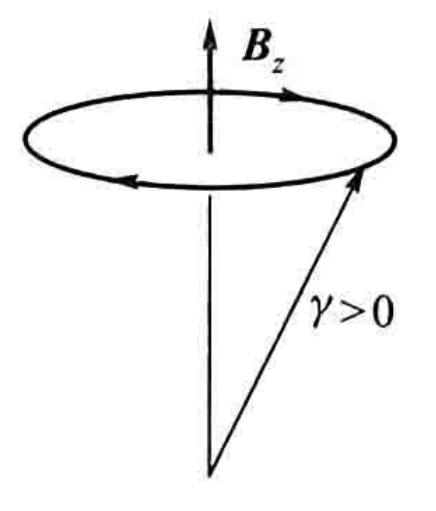
\includegraphics[width=0.2\linewidth]{fig/precession.png}
  \caption{磁矩在外场下Larmor进动的半经典图像}
  \label{fig:precession}
\end{figure}

宏观上,样品磁化强度是众多微观磁矩之和:$\bm{M} = \sum_i \bm{\mu}_i$, 这也是实际测量的物理量;粒子数在上、下能级的分布大致为Boltzmann分布,能级间的粒子数差异$n_0$是观测到共振现象的关键。处于热平衡时,$M_{x0}=M_{y0}=0$,$M_{z0}=M_0$。若通过某种途径使得$M_{x},M_{y},M_{z}$偏离平衡数值,此时就存在着使得$M_{x},M_{y},M_{z}$趋向热平衡的自发过程,称为弛豫过程。$M_{x},M_{y},M_{z}$的自发弛豫过程遵循下面的规律
\begin{equation}
  \left\{\begin{aligned}
    &\frac{\d M_z}{\d t}=-\frac{1}{T_1}(M_z-M_0),\\
    &\frac{\d M_x}{\d t}=-\frac{1}{T_2}M_x,\\
    &\frac{\d M_y}{\d t}=-\frac{1}{T_2}M_y.
  \end{aligned}\right.
\end{equation}其中$T_1$被称为纵向弛豫时间,主要来自于自旋-晶格相互作用;而$T_2$被称为横向弛豫时间,主要来自于自旋-自旋相互作用。若同时引入外磁场和弛豫作用,就可以写下描述核磁共振现象的基本方程式——布洛赫方程式(参见教材\cite{book})。通过求解这个方程式,我们就可以解释各种磁共振现象。
	
最后注意;引入射频场后,当射频场作用与自旋--晶格驰豫达到动态平衡时,$n < n_0$. 特别当扰动场强$B_1$很大时,共振吸收过强,此时能级间粒子数差异$n\to 0$, 出现饱和现象,难以观测到共振吸收,因此$B_1$不能过大。

\section{实验装置}
\begin{figure}
\centering
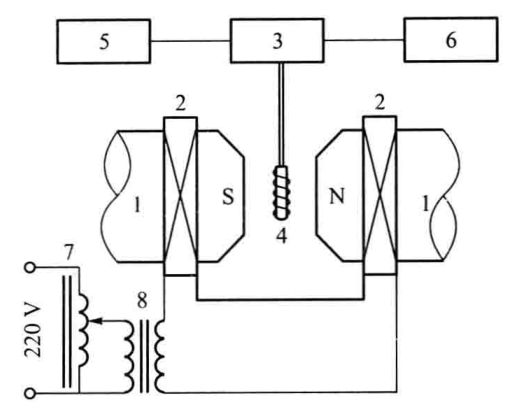
\includegraphics[width=0.4\linewidth]{fig/apparatus.png}
\caption{核磁共振装置示意图。恒定磁场及扫场信号沿图示水平方向,恒磁场在均匀区范围内均匀性优于$10^{-5}$。射频信号的产生与共振信号的接收均通过边限振荡器实现。1——永久磁铁;2——扫场线圈;3——电路盒;4——样品和震荡线圈;5——数字频率计;6——示波器;7——可调变压器;8——220 V/6 V变压器。}
\label{fig:apparatus}
\end{figure}

实验采用NM-3型核磁共振装置,其工作原理如\autoref{fig:apparatus} 所示。

射频磁场由振荡线圈(边限振荡器)产生,其产生的线偏振磁场可以分解为左旋、右旋圆偏振场,其中一个圆偏成分使样品共振激发;另一圆偏成分频率相反,远离共振区,其影响可以忽略。

实验中须使系统参数渐变地通过共振区间,以观察共振峰;若仅调整射频场频率而固定$B_0$不变,由于射频场频率旋钮的调节步长难以控制,远大于共振线宽,故极易错过共振区间。
	
因此,实验中利用电磁铁在$B_0$上附加一个共线的50 Hz交变磁场,相当于使恒磁场在$B_0 \pm\Delta B$之间连续变化,称为扫场。给定射频场频率,只要共振条件对应的场强在扫场变化范围内,就能观察到共振信号(这里的扫场频率不能太太,以至于整个系统在每个时刻都可以近似看作在恒定不变的磁场下)。

\section{实验结果与分析}
\subsection{观察掺有FeCl$_3$的水样品中质子的共振信号}
样品置于磁场中央,调整扫场电压$\sim$100 V,调整射频场频率直到示波器上可见共振峰,之后再调节幅度和样品位置,在保持频率不变的情况下使得共振信号最大。随后,我们改变(1)射频场的频率;(2)扫场幅度;(3)电路盒在磁铁上方平台的左右位置;(4)改变射频场的幅度,观察共振信号的波形、幅度和位置分布等因素的变化并做出简单分析。
\begin{enumerate}
  \item 增大射频场$B_1$的频率,观察共振信号。
  \begin{itemize}
  \item \textbf{波形}:首先可见微弱的正弦背景,在射频场频率接近核磁共振频率的时候会出现共振峰,出现共振峰后,峰的右侧立即可见密集的尾波,一直如此直到共振信号消失;尾波的变化并不显著。共振信号存在的射频场频率范围为[21.019 MHz, 21.188MHz]。
  \item \textbf{幅度}:出现信号后迅速增大,随后渐减至稳定(此时共振信号等间距);随后又渐增,在信号合二为一后骤减消失。
  \item \textbf{位置}:在增大射频场频率的过程中,波谷首先出现共振信号峰,随后共振峰一分为二,直至以10 ms的间隔等间距分布(此时射频场频率为$\nu_0$=21.103 MHz)。随后又逐渐两两靠近,最终合二为一后消失。信号消失在正弦背景的波峰附近。
  \end{itemize}
\textbf{分析}:这正是射频场频率通过$B_0\pm\Delta B$共振区间的过程,其中微弱的正弦背景正是扫场信号。随射频场频率增大,$B_0+\Delta B$首先满足共振条件,所以共振峰会先出现在正弦背景的波峰处。随后在每个扫场周期中,有2个磁场值满足共振条件,故有共振峰一分为二。在$B_0-\Delta B$时最后满足共振条件,所以共振峰会最后在正弦背景的波谷处合二为一并消失。两共振峰接近时互相增强,因此幅度大。特别地,当共振峰等10 ms间距时,对应的共振磁场大致是$B_0$。\par
尾波是共振激发后感生电动势频率与射频场频率间微小不同所造成的拍现象。而且有效驰豫时间$T$越短,暂态现象越不明显;而磁场的不均匀性将使$T$值减小,故外磁场越均匀,尾波频次越多;可由此判断磁场均匀性。此外,尾波还和扫场速度有关,如\autoref{fig:tail} 所示,不同的扫场次数会导致不同的尾波振荡次数。
\begin{figure}
  \centering
  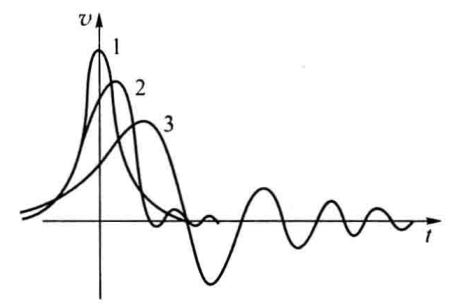
\includegraphics[width=0.4\linewidth]{fig/tail.png}
  \caption{扫场速度不同时所观察到的核磁共振吸收信号。1——扫场速度趋于零;2——扫场速度中等;3——扫场速度较快。}
  \label{fig:tail}
\end{figure}
\item 将扫场电压调至$\sim$200 V,增大射频场频率,观察共振信号。
  \begin{itemize}
  \item \textbf{波形}:正弦背景增强,共振信号存在的射频场范围增大,为[20.940 MHz, 21.267MHz]。尾波相对于100 V扫场电压的情形更加明显。
  \item \textbf{幅度}:共振幅度相比于较低的扫场电压增大。
  \item \textbf{位置}:位置相对于上一种情形并没有显著变化。
  \end{itemize}
  \textbf{分析}:
  增大扫场电压就是增大了$B_0$的变化范围$\Delta B$,因此正弦背景增强。而这会导致在更大的频率范围$\Delta \nu$内可以观察到共振现象。\par
  尾波实际上是共振频率与射频场频率有微小差异时的拍现象;$\Delta B$变大即增加了共振频范围$\Delta\nu$, 频率相差越远,拍频越大,即尾波越密。
\item 将扫场电压调至$\sim$50 V,增大射频场频率,观察共振信号。
\begin{itemize}
  \item \textbf{波形}:正弦背景减弱,共振信号存在的射频场范围减小,为[21.056 MHz, 21.146MHz]。尾波相对于100 V扫场电压的情形更不明显。
  \item \textbf{幅度}:共振幅度相比于较高的扫场电压减小。
  \item \textbf{位置}:位置相对于上一种情形并没有显著变化。
\end{itemize}
\textbf{分析}:和第2中情形的分析类似。
\item 将扫场电压调至100 V, 调射频场频率使共振信号以10 ms等间距分布,从最右端到最左端移动样品。
  \begin{itemize}
  \item \textbf{波形}:最先没有尾波,随后出现疏且少的尾波,逐渐变密变多,最多在1.9 cm刻度附近;此后又渐疏渐少至消失。
  \item \textbf{幅度}:先增大后减小,最大幅度在1.9 cm刻度附近。
  \item \textbf{位置}:无明显变化。
  \end{itemize}
  \textbf{分析}:左右移动样品相当于改变$B_0$的强度和均与性;在两侧$B_0$弱且不均匀,故共振峰幅度小。此外,如前所述,$B_0$的不均匀性将减小等效驰豫时间$T$, 这不利于尾波的形成,故样品在两侧时不可见尾波。由此可知,1.9 cm刻度附近的磁场最为均匀。
\item 样品重新置于1.9 cm刻度处,扫场电压调至100 V。由小到大调整其幅度,并始终保持射频场频率不变。
  \begin{itemize}
  \item \textbf{波形}:无明显变化。
  \item \textbf{幅度}:先增大后减小,最大在射频场幅度6至7刻度附近(这里可能存在一定误差,因为在幅度变化的中段,信号的幅度变化并不明显)。
  \item \textbf{位置}:无明显变化。事实上,实验中调整射频场幅度后其频率会发生漂移,正是通过进一步的调整信号以10 ms等间距分布以控制射频场频率不变。
  \end{itemize}
  \textbf{分析}:射频场较小时,幅度越大共振跃迁越显著,对应信号幅度增大;射频场过大时,发生饱和现象,信号幅度反之减小。
\end{enumerate}
\subsection{利用核磁共振校准磁场}
在前述实验所确定的最优参数下,利用前述减小扫场幅度的手段控制精度,以校准$B_0$.具体而言,给定质子的回旋频率
\begin{equation}
  \frac{\gamma}{2\pi}=\num{ 42.5763888} \pm \SI{ 0.0000018}{\MHz/T},
\end{equation}利用共振条件\autoref{eq:resonance_simplified} 及$\Delta B$确定$B_0$及其不确定度。实际测量时,当共振峰以10 ms等间距分布时,对应的共振频率是
	\begin{equation}
		\nu_0 = \SI{21.10318}{\MHz},
	\end{equation}
	估测频率的不确定度为$\sigma_{\nu_0}\approx 0.001\ {\rm MHz}$(实际测量时,在0.001 MHz的射频场频率变化范围内,难以区分共振信号的变化),这给出磁场的不确定度估计
	\begin{equation}
		\sigma_{B_0} = B_0\sqrt{\left(\frac{\sigma_{\gamma}}{\gamma}\right)^2+\left(\frac{\sigma_{\nu_0}}{\nu_0}\right)^2}.
	\end{equation}
	综上,可以计算得到永久磁铁的磁场为
	\begin{equation}
		B_0 = (\num{0.49565}\pm \num{0.00002})\ {\rm T}.
	\end{equation}
	相对不确定度为
\begin{equation}
  \frac{\sigma_{B_0}}{B_0}\approx5\times10^{-5}.
\end{equation}

\subsection{测量四氟乙烯中氟核的朗德$g$因子}
类似上面做过的调节,利用已经校准的$B_0$, 可测定未知氟核的$g$因子。对于聚四氟乙烯中的氟核,已知共振频率$\nu_0$, 由共振条件\autoref{eq:resonance_simplified} 有\begin{equation}g = \frac{\nu_0/B_0}{\mu_N/h},\end{equation} 其中
\begin{equation}
  \frac{\mu_N}{h}=7.622\ 593\ 96\pm\SI{ 0.00000031}{\MHz/T}.
\end{equation}
测量得到共振频率为
\begin{equation}
  \nu_0 = \SI{19.85325}{\MHz}.
\end{equation}
估测频率的不确定度为$\sigma_{\nu}\approx 0.001\ {\rm MHz}$,这给出氟核朗德$g$因子测量的不确定度估计
\begin{equation}
  \sigma_{g} = g\sqrt{\left(\frac{\sigma_{B_0}}{B_0}\right)^2+\left(\frac{\sigma_{\nu_0}}{\nu_0}\right)^2+\left(\frac{\sigma_{\mu_N}}{\mu_N}\right)^2}.
\end{equation}
综上,可以计算得到氟核的朗德$g$因子为
\begin{equation}
  g = \num{5.2548}\pm\num{0.0003}.
\end{equation}
相对不确定度为
\begin{equation}
  \frac{\sigma_{g}}{g}\approx6\times10^{-5}.
\end{equation}
\subsection{测量四氟乙烯中氟核的横向弛豫时间$T_2$}
将底座前方“扫场输出”的信号输入到X端,“检波输出”信号输入到Y端,示波器用X-Y输入方法。适当调大扫场幅度至200 V,在上面已经调节好的共振频率下,从示波器上观察到的是重叠而又相错开的两个峰(可以利用相移调节旋钮改变两个峰的位置)。

用网格估计其中一个共振峰的半宽$\Delta B$和扫场变化范围$2B'$的比值
	\begin{equation}
		\kappa =\frac{\Delta B}{2B'}=\frac{U_{\Delta B}}{U_{2B'}} = \frac{0.28\ {\rm V}}{6.85\ {\rm V}}\approx 0.0409.
	\end{equation}
测量共振发生在扫场的峰顶和谷底时的共振频率,得到\begin{equation}
  \begin{aligned}
    &v_{F\min}=\SI{19.68344}{\MHz},\\
    &v_{F\max}=\SI{19.98640}{\MHz}.
  \end{aligned}
\end{equation}
因为$\frac12\Delta\omega\sim\frac{1}{T_2}$,所以横向弛豫时间$T_2$可由下面式子得到
\begin{equation}
  T_2\approx\frac{1}{\pi\kappa(v_{F\max}-v_{F\min})},
\end{equation}

最终,计算得到氟核的横向弛豫时间为
\begin{equation}
  T_2\approx25.7\ {\rm \mu s}.
\end{equation}

\subsection{观察纯水样品(不含FeCl$_3$)的核磁共振现象}\label{pure_w}
在第一部分实验中,水样品掺有FeCl$_3$, 作为比较,实验中最后观测了纯水样品的核磁共振现象;相对掺有FeCl$_3$的水而言,纯水样品的共振信号极弱。在对掺有FeCl$_3$的水而言的最佳实验条件下,纯水样品难以看到共振峰,唯有当射频场幅度调至最高时才勉强可以看见信号(将示波器的分辨率调节到2 mV时可以看到)。共振频率在25 MHz附近。这是因为样品由于掺入顺磁剂Fe$^{3+}$离子,使样品中局域磁场增强,显著减小了样品的驰豫时间,从而使得共振峰得以增强。
\section{结论}
通过本实验,我们系统地研究了核磁共振现象,观察并分析了实验参数对核磁共振信号的影响,找出了最佳的测定条件,调节合适的扫场幅度大小、均匀且恒强的静磁场及适当的射频场频率。这些条件为我们提供了观察到核磁共振信号的基础。在此基础之上,我们成功地通过核磁共振校准了磁场,并精确测定了聚四氟乙烯中氟核的$g$因子及横向驰豫时间。这些结果不仅验证了核磁共振在精密测量中的有效性,也为我们进一步探索核磁共振现象提供了坚实的实验基础和数据支持。总的来说,本实验深化了我们对核磁共振现象的理解,并为其在未来的精密测量应用中提供了重要的实践经验和理论依据。

\begin{thebibliography}{}
  \bibitem{rabi1938new} Rabi, Isidor I., Zacharias, Jerrold R., Millman, Sidney, Kusch, Polykarp. (1938). A new method of measuring nuclear magnetic moment. \textit{Physical review. 53(4)}, 318.
  \bibitem{book} 吴思诚, 荀坤. (2015). 近代物理实验(第四版). 北京: 高等教育出版社.
\end{thebibliography}
  
\clearpage % 附录前另起一页
\appendix % 附录开始
\section{思考题}
\subsection{对“纯水”样品与掺有三氯化铁的“水”样品中质子共振信号的主要差别做出解释。}
如\autoref{pure_w} 中分析,由于样品掺入顺磁剂Fe$^{3+}$离子,使样品中局域磁场增强,显著减小了样品的驰豫时间,从而使得共振峰得以显著增强。

\section{实验记录本}
实验记录本。
\end{document}
